%%%%%%%%%%%%%%%%%%%%%%%%%%%%%%%%%%%%%%%%%
% Jacobs Landscape Poster
% LaTeX Template
% Version 1.1 (14/06/14)
%
% Created by:
% Computational Physics and Biophysics Group, Jacobs University
% https://teamwork.jacobs-university.de:8443/confluence/display/CoPandBiG/LaTeX+Poster
% 
% Further modified by:
% Nathaniel Johnston (nathaniel@njohnston.ca)
%
% This template has been downloaded from:
% http://www.LaTeXTemplates.com
%
% License:
% CC BY-NC-SA 3.0 (http://creativecommons.org/licenses/by-nc-sa/3.0/)
%
%%%%%%%%%%%%%%%%%%%%%%%%%%%%%%%%%%%%%%%%%

%----------------------------------------------------------------------------------------
%	PACKAGES AND OTHER DOCUMENT CONFIGURATIONS
%----------------------------------------------------------------------------------------

\documentclass[final]{beamer}
\documentclass[12pt,twoside,a4paper,openright]{report}
\usepackage{etex}
% Select encoding of your inputs.
\usepackage[utf8]{inputenc}

% Make latex understand and use the typographic
% rules of the language used in the document.
\usepackage[english, danish]{babel}

% Use the vector font Latin Modern which is going
% to be the default font in latex in the future.
\usepackage{lmodern}

% Choose the font encoding
\usepackage[T1]{fontenc}

% Use colour in tables
\usepackage[table]{xcolor}
\usepackage{array}
\usepackage{multirow}

% load a colour package
\usepackage{xcolor}
\definecolor{aaublue}{RGB}{33,26,82}% dark blue

% The standard graphics inclusion package
\definecolor{white}{RGB}{255,255,255} % define color white
\usepackage{graphicx}
\usepackage{adjustbox}

% Set up how figure and table captions are displayed
\usepackage{caption}
\captionsetup{
  font=footnotesize,% set font size to footnotesize
  labelfont=bf % bold label (e.g., Figure 3.2) font
}

% Enable row combination in tables
\usepackage{multirow}

% Make space between table lines and text
\renewcommand{\arraystretch}{1.5}

% Make the standard latex tables look so much better
\usepackage{array,booktabs}

% Enable the use of frames around, e.g., theorems
% The framed package is used in the example environment
\usepackage{framed}
\usepackage{colortbl}
\usepackage{longtable}
\usepackage{xcolor}
\usepackage{textcomp}

%%%%%%%%%%%%%%%%%%%%%%%%%%%%%%%%%%%%%%%%%%%%%%%%
% Mathematics
%%%%%%%%%%%%%%%%%%%%%%%%%%%%%%%%%%%%%%%%%%%%%%%%
% Defines new environments such as equation,
% align and split 
\usepackage{amsmath}
\usepackage{relsize}
% Adds new math symbols
\usepackage{amssymb}
% Use theorems in your document
% The ntheorem package is also used for the example environment
% When using thmmarks, amsmath must be an option as well. Otherwise \eqref doesn't work anymore.
\usepackage[framed,amsmath,thmmarks]{ntheorem}
\usepackage{cancel}

%%%%%%%%%%%%%%%%%%%%%%%%%%%%%%%%%%%%%%%%%%%%%%%%
% Page Layout
%%%%%%%%%%%%%%%%%%%%%%%%%%%%%%%%%%%%%%%%%%%%%%%%
% Change margins, papersize, etc of the document
\usepackage[
  left=25mm,% left margin on an odd page %tidligere 25mm for baade right og left
  right=25mm,% right margin on an odd page
  top=35mm,
  ]{geometry}
  
% Modify how \chapter, \section, etc. look
% The titlesec package is very configureable
\usepackage{titlesec}
\makeatletter
\def\ttl@mkchap@i#1#2#3#4#5#6#7{%
    \ttl@assign\@tempskipa#3\relax\beforetitleunit
    \vspace{\@tempskipa}%<<<<<< REMOVE THE * AFTER \vspace
    \global\@afterindenttrue
    \ifcase#5 \global\@afterindentfalse\fi
    \ttl@assign\@tempskipb#4\relax\aftertitleunit
    \ttl@topmode{\@tempskipb}{%
        \ttl@select{#6}{#1}{#2}{#7}}%
    \ttl@finmarks  % Outside the box!
    \@ifundefined{ttlp@#6}{}{\ttlp@write{#6}}}
\makeatother

\titlespacing{\chapter}{0pt}{0pt}{10pt}
\titlespacing{\section}{0pt}{0pt}{-5pt}
\titlespacing{\subsection}{0pt}{8pt}{-5pt}
\titlespacing{\subsubsection}{0pt}{6pt}{-10pt}

\titleformat*{\section}{\normalfont\Large\bfseries\color{aaublue}}
\titleformat*{\subsection}{\normalfont\large\bfseries\color{aaublue}}
\titleformat*{\subsubsection}{\normalfont\normalsize\bfseries\color{aaublue}}

\usepackage{bookmark}
\usepackage{titlesec, blindtext, color}
%\color{gray75}{gray}{0.75}
\newcommand{\hsp}{\hspace{20pt}}
\titleformat{\chapter}[hang]{\Huge\bfseries}{\thechapter\hsp\textcolor{aaublue}{|}\hsp}{0pt}{\Huge\bfseries}

% Change the headers and footers
\usepackage{fancyhdr}
\setlength{\headheight}{15pt}
\pagestyle{fancy}
\fancyhf{} %delete everything
\renewcommand{\headrulewidth}{0pt} %remove the horizontal line in the header
\fancyhead[RO,LE]{\color{aaublue}\small\nouppercase\leftmark} %even page - chapter title
\fancyhead[LO]{}
\fancyhead[RE]{} 
\fancyhead[CE]{}
\fancyhead[CO]{}
\fancyfoot[RE,LO]{\thepage}
\fancyfoot[LE,RO]{} %page number on all pages
\fancyfoot[CE,CO]{}

% change first page of all chapters header and footer to fancy style
\makeatletter
\let\ps@plain\ps@fancy
\makeatother

% Do not stretch the content of a page. Instead,
% insert white space at the bottom of the page
\raggedbottom

% Enable arithmetics with length. Useful when typesetting the layout.
\usepackage{calc}

%%%%%%%%%%%%%%%%%%%%%%%%%%%%%%%%%%%%%%%%%%%%%%%%
% Bibliography
%%%%%%%%%%%%%%%%%%%%%%%%%%%%%%%%%%%%%%%%%%%%%%%%
%setting references (using numbers) and supporting i.a. Chicargo-style:
\usepackage{etex}
\usepackage{etoolbox}
\usepackage{keyval}
\usepackage{ifthen}
\usepackage{url}
\usepackage{csquotes}
\usepackage[backend=biber, url=true, doi=true, style=numeric, sorting=none]{biblatex}
\addbibresource{setup/bibliography.bib}

%%%%%%%%%%%%%%%%%%%%%%%%%%%%%%%%%%%%%%%%%%%%%%%%
% Misc
%%%%%%%%%%%%%%%%%%%%%%%%%%%%%%%%%%%%%%%%%%%%%%%%

%%% Enables the use FiXme refferences. Syntax: \fxnote{...} %%%
\usepackage[footnote, draft, english, silent, nomargin]{fixme}
%With "final" instead of "draft" an error will ocure for every FiXme under compilation.

%%% allows use of lorem ipsum (generate i.e. pagagraph 1 to 5 with \lipsum[1-5]) %%%
\usepackage{lipsum}

%%% Enables figures with text wrapped tightly around it %%%
\usepackage{wrapfig}

%%% Section debth included in table of contents (1 = down to sections) %%%
\setcounter{tocdepth}{1}

%%% Section debth for numbers (1 = down to sections) %%%
\setcounter{secnumdepth}{1}

\usepackage{tocloft}
\setlength{\cftbeforetoctitleskip}{0 cm}
\renewcommand{\cftpartpresnum}{Part~}
\let\cftoldpartfont\cftpartfont
\renewcommand{\cftpartfont}{\cftoldpartfont\cftpartpresnum}

%%%%%%%%%%%%%%%%%%%%%%%%%%%%%%%%%%%%%%%%%%%%%%%%
% Hyperlinks
%%%%%%%%%%%%%%%%%%%%%%%%%%%%%%%%%%%%%%%%%%%%%%%%

% Enable hyperlinks and insert info into the pdf
% file. Hypperref should be loaded as one of the 
% last packages
\usepackage{nameref}
\usepackage{hyperref}
\hypersetup{%
	%pdfpagelabels=true,%
	plainpages=false,%
	pdfauthor={Author(s)},%
	pdftitle={Title},%
	pdfsubject={Subject},%
	bookmarksnumbered=true,%
	colorlinks,%
	citecolor=aaublue,%
	filecolor=aaublue,%
	linkcolor=aaublue,% you should probably change this to black before printing
	urlcolor=aaublue,%
	pdfstartview=FitH%
}

% remove all indentations
\setlength\parindent{0pt}
\parskip 5mm
\usepackage{verbatim}

\definecolor{Gra}{RGB}{230,230,230}

%creates a nice-looking C#-text
\newcommand{\CC}{C\nolinebreak\hspace{-.05em}\raisebox{.3ex}{\scriptsize\text \#} }

%enables multi column lists
\usepackage{multicol}

%enables code-examples
\usepackage{listings}

\definecolor{coolblue}{RGB}{32,95,128}
\definecolor{mygreen}{rgb}{0,0.6,0}
\definecolor{mygray}{rgb}{0.5,0.5,0.5}
\definecolor{mymauve}{rgb}{0.58,0,0.82}
\usepackage{textcomp}
\definecolor{listinggray}{gray}{0.9}
\definecolor{lbcolor}{rgb}{0.9,0.9,0.9}

\lstdefinestyle{customcpp}{
    backgroundcolor=\color{lbcolor},
    tabsize=4,
    rulecolor=,
    language=C++,
    basicstyle=\scriptsize,
    upquote=true,
    aboveskip={1.5\baselineskip},
    columns=fixed,
    showstringspaces=false,
    extendedchars=true,
    breaklines=true,
    prebreak = \raisebox{0ex}[0ex][0ex]{\ensuremath{\hookleftarrow}},
    frame=single,
    showtabs=false,
    numbers=left,
    captionpos=b,
    numbersep=5pt,
    numberstyle=\tiny\color{mygray},
    showspaces=false,
    showstringspaces=false,
    identifierstyle=\ttfamily,
    keywordstyle=\color[rgb]{0,0,1},
    commentstyle=\color[rgb]{0.133,0.545,0.133},
    stringstyle=\color[rgb]{0.627,0.126,0.941},
}
\lstdefinestyle{custommatlab}{
    backgroundcolor=\color{lbcolor},
    tabsize=4,
    rulecolor=,
    language=Matlab,
    basicstyle=\scriptsize,
    upquote=true,
    aboveskip={1.5\baselineskip},
    columns=fixed,
    showstringspaces=false,
    extendedchars=true,
    breaklines=true,
    prebreak = \raisebox{0ex}[0ex][0ex]{\ensuremath{\hookleftarrow}},
    frame=single,
    showtabs=false,
    numbers=left,
    captionpos=b,
    numbersep=5pt,
    numberstyle=\tiny\color{mygray},
    showspaces=false,
    showstringspaces=false,
    identifierstyle=\ttfamily,
    keywordstyle=\color[rgb]{0,0,1},
    commentstyle=\color[rgb]{0.133,0.545,0.133},
    stringstyle=\color[rgb]{0.627,0.126,0.941},   
}
\lstdefinestyle{custommatlabinline}{
    style=custommatlab,
    basicstyle=\small,
}
\lstdefinestyle{customcppinline}{
    style=customcpp,
    basicstyle=\small,
}
\lstset{
%  backgroundcolor=\color{white},   % choose the background color; you must add \usepackage{color} or \usepackage{xcolor}
%  basicstyle=\footnotesize,        % the size of the fonts that are used for the code
%  breakatwhitespace=false,         % sets if automatic breaks should only happen at whitespace
%  breaklines=true,                 % sets automatic line breaking
%  captionpos=t,                    % sets the caption-position to bottom
%  commentstyle=\color{mygreen},    % comment style
%  deletekeywords={...},            % if you want to delete keywords from the given language
%  escapeinside={\%*}{*)},          % if you want to add LaTeX within your code
%  extendedchars=true,              % lets you use non-ASCII characters; for 8-bits encodings only, does not work with UTF-8
%  frame=single,                    % adds a frame around the code
%  keepspaces=true,                 % keeps spaces in text, useful for keeping indentation of code (possibly needs columns=flexible)
%  keywordstyle=\color{blue},       % keyword style
%  language=C++,                 % the language of the code
%  morekeywords={*,...},            % if you want to add more keywords to the set
%  numbers=left,                    % where to put the line-numbers; possible values are (none, left, right)
%  numbersep=5pt,                   % how far the line-numbers are from the code
%  numberstyle=\tiny\color{mygray}, % the style that is used for the line-numbers
%  rulecolor=\color{black},         % if not set, the frame-color may be changed on line-breaks within not-black text (e.g. comments (green here))
%  showspaces=false,                % show spaces everywhere adding particular underscores; it overrides 'showstringspaces'
%  showstringspaces=false,          % underline spaces within strings only
%  showtabs=false,                  % show tabs within strings adding particular underscores
%  stepnumber=1,                    % the step between two line-numbers. If it's 1, each line will be numbered
%  stringstyle=\color{mymauve},     % string literal style
%  tabsize=2,                       % sets default tabsize to 2 spaces
%  title=\lstname                   % show the filename of files included with \lstinputlisting; also try caption instead of title
    style=customcpp
}

\usepackage{float}
\usepackage{caption}
\usepackage{subcaption}
\usepackage{siunitx}
\sisetup{decimalsymbol=comma}
\sisetup{detect-weight}

\usepackage{enumitem}
%\usepackage[citestyle=authoryear,natbib=true]{biblatex}

% Figures - TIKZ
\usepackage{tikz}
\usetikzlibrary{shapes,arrows}
\usepackage[americanresistors,americaninductors,americancurrents, americanvoltages]{circuitikz}

% Wall of text logo
\newcommand{\walloftextalert}[0]{\includegraphics[width=\textwidth]{walloftext.png}}

\usepackage{pdfpages}
\usepackage{lastpage}
\usepackage{epstopdf}

\setlength{\headheight}{21pt}

\hfuzz=\maxdimen
\tolerance = 10000
\hbadness  = 10000

\usepackage{siunitx}
\graphicspath{{./figures/}}% package inclusion and set up of the document

%%%%%%%%%%%%%%%%%%%%%%%%%%%%%%%%%%%%%%%%%%%%%%%%%%%%%
%             UNITS, EQUATIONS AND TEXT             %
%%%%%%%%%%%%%%%%%%%%%%%%%%%%%%%%%%%%%%%%%%%%%%%%%%%%%
%Units:
\newcommand{\unit}[1]{&& \left[\si{#1}\right]} %\newcommand{\unit}[1]{[\si{#1}]}             <<| Use these if you want equations to be
\newcommand{\unitWh}[1]{[\si{#1}]}             %\newcommand{\eq}[2]{&&\si{#1} &= \si{#2}&&}  <<| centered.. .. will appear scrambled
\newcommand{\numUnit}[1]{\ \si{#1}&}           %                                               | from one equation to the next though..
%Equation:                                     %                                               | and does not work with long equations.. :/
\newcommand{\eq}[2]{\si{#1} &= \si{#2}}
\newcommand{\arw}{&& &\Updownarrow&&}
\newcommand{\eqOne}[2]{\si{#1} &= \si{#2} &\nonumber\\}
\newcommand{\eqTwo}[1]{&\ \ \ \ \si{#1}&}
%Text:
\newcommand{\tx}[1]{\text{#1}}
%Vectors
\renewcommand{\vec}[1]{\boldsymbol{\mathbf{#1}}}
%Vertical line in equations ie. |_x=y (whereTwo stacks two equalities at the line)
\newcommand{\where}[1]{ \left.\rule{0cm}{.5cm}\right\vert\rule{0cm}{.4cm}_{\substack{\rule{0cm}{.15cm}\\ \si{#1} }} }
\newcommand{\whereTwo}[2]{ \left.\rule{0cm}{.67cm}\right\vert\rule{0cm}{.5cm}_{\substack{\si{#1} \rule{0cm}{.19cm}\\\vspace{-.1cm}\\ \si{#2}}} }

%%%%%%%%%%%%%%%%%%%%%%%%%%%%%%%%%%%%%%%%%%%%%%%%%%%%%
%                 TIKZ SETTINGS                     %
%%%%%%%%%%%%%%%%%%%%%%%%%%%%%%%%%%%%%%%%%%%%%%%%%%%%%
\usetikzlibrary{arrows.meta}
\tikzset{
  block/.style    = {draw, thick, rectangle,
                     minimum height = 2.1em,
                     minimum width = 1.7em},
  sum/.style      = {draw, circle, inner sep=1.5pt},
}

%%%%%%%%%%%%%%%%%%%%%%%%%%%%%%%%%%%%%%%%%%%%%%%%%%%%%
%                  REFERENCES                       %
%%%%%%%%%%%%%%%%%%%%%%%%%%%%%%%%%%%%%%%%%%%%%%%%%%%%%

%Chapter
\newcommand{\Chapref}[1]{\emph{Chapter \ref{#1}}}
\newcommand{\chapref}[1]{\emph{chapter \ref{#1}}}
%Section
\newcommand{\Secref}[1]{\emph{Section \ref{#1}}}
\newcommand{\secref}[1]{\emph{section \ref{#1}}}
%subSection
\newcommand{\Subsecref}[1]{\emph{Subsection \ref{#1}}}
\newcommand{\subsecref}[1]{\emph{subsection \ref{#1}}}
%Appendix
\newcommand{\Appref}[1]{\emph{Appendix \ref{#1}}}
\newcommand{\appref}[1]{\emph{appendix \ref{#1}}}
%Listings
\newcommand{\Coderef}[1]{\emph{Listings: \ref{#1}}}
\newcommand{\coderef}[1]{\emph{listings: \ref{#1}}}
%Figure:
\newcommand{\Figref}[1]{\emph{Figure \ref{#1}}}
\newcommand{\figref}[1]{\emph{figure \ref{#1}}}
%Table:
\newcommand{\Tableref}[1]{\emph{Table \ref{#1}}}
\newcommand{\tableref}[1]{\emph{table \ref{#1}}}

%Expressions:
\newcommand{\Expr}[1]{\emph{Expression (\ref{#1})}}
\newcommand{\expr}[1]{\emph{expression (\ref{#1})}}

%Equations:
%1 equation:
\newcommand{\Eqref}[1]{\emph{Equation (\ref{#1})}}
\renewcommand{\eqref}[1]{\emph{equation (\ref{#1})}}
%2 equations:
\newcommand{\EqrefTwo}[2]{\emph{Equation (\ref{#1})} and \emph{(\ref{#2})}}
\newcommand{\eqrefTwo}[2]{\emph{equation (\ref{#1})} and \emph{(\ref{#2})}}
%3 equations:
\newcommand{\EqrefThree}[3]{\emph{Equation (\ref{#1})}, \emph{(\ref{#2})} and \emph{(\ref{#3})}}
\newcommand{\eqrefThree}[3]{\emph{equation (\ref{#1})}, \emph{(\ref{#2})} and \emph{(\ref{#3})}}
%4 equations:
\newcommand{\EqrefFour}[4]{\emph{Equation (\ref{#1})}, \emph{(\ref{#2})}, \emph{(\ref{#3})} and \emph{(\ref{#4})}}
\newcommand{\eqrefFour}[4]{\emph{equation (\ref{#1})}, \emph{(\ref{#2})}, \emph{(\ref{#3})} and \emph{(\ref{#4})}}
%5 equations:
\newcommand{\EqrefFive}[5]{\emph{Equation (\ref{#1})}, \emph{(\ref{#2})}, \emph{(\ref{#3})}, \emph{(\ref{#4})} and \emph{(\ref{#5})}}
\newcommand{\eqrefFive}[5]{\emph{equation (\ref{#1})}, \emph{(\ref{#2})}, \emph{(\ref{#3})}, \emph{(\ref{#4})} and \emph{(\ref{#5})}}
%6 equations:
\newcommand{\EqrefSix}[6]{\emph{Equation (\ref{#1})}, \emph{(\ref{#2})}, \emph{(\ref{#3})}, \emph{(\ref{#4})}, \emph{(\ref{#5})} and \emph{(\ref{#6})}}
\newcommand{\eqrefSix}[6]{\emph{equation (\ref{#1})}, \emph{(\ref{#2})}, \emph{(\ref{#3})}, \emph{(\ref{#4})}, \emph{(\ref{#5})} and \emph{(\ref{#6})}}
%7 equations:
\newcommand{\EqrefSeven}[7]{\emph{Equation (\ref{#1})}, \emph{(\ref{#2})}, \emph{(\ref{#3})}, \emph{(\ref{#4})}, \emph{(\ref{#5})}, \emph{(\ref{#6})} and \emph{(\ref{#7})}}
\newcommand{\eqrefSeven}[7]{\emph{equation (\ref{#1})}, \emph{(\ref{#2})}, \emph{(\ref{#3})}, \emph{(\ref{#4})}, \emph{(\ref{#5})}, \emph{(\ref{#6})} and \emph{(\ref{#7})}}% my new macros

\usepackage[scale=1.24]{beamerposter} % Use the beamerposter package for laying out the poster

\usetheme{confposter} % Use the confposter theme supplied with this template

%\setbeamercolor{block title}{fg=black,bg=white} % Colors of the block titles
%\setbeamercolor{block body}{fg=black,bg=white} % Colors of the body of blocks
%\setbeamercolor{block alerted title}{fg=white,bg=dblue!70} % Colors of the highlighted block titles
\setbeamercolor{block alerted body}{fg=black,bg=white} % Colors of the body of highlighted blocks
% Many more colors are available for use in beamerthemeconfposter.sty

%-----------------------------------------------------------
% Define the column widths and overall poster size
% To set effective sepwid, onecolwid and twocolwid values, first choose how many columns you want and how much separation you want between columns
% In this template, the separation width chosen is 0.024 of the paper width and a 4-column layout
% onecolwid should therefore be (1-(# of columns+1)*sepwid)/# of columns e.g. (1-(4+1)*0.024)/4 = 0.22
% Set twocolwid to be (2*onecolwid)+sepwid = 0.464
% Set threecolwid to be (3*onecolwid)+2*sepwid = 0.708

\newlength{\sepwid}
\newlength{\onecolwid}
\newlength{\twocolwid}
\newlength{\threecolwid}
\setlength{\paperwidth}{48in} % A0 width: 46.8in
\setlength{\paperheight}{36in} % A0 height: 33.1in
\setlength{\sepwid}{0.01\paperwidth} % Separation width (white space) between columns
\setlength{\onecolwid}{0.22\paperwidth} % Width of one column
\setlength{\twocolwid}{0.52\paperwidth} % Width of two columns
\setlength{\threecolwid}{0.708\paperwidth} % Width of three columns (not used in this poster)
\setlength{\topmargin}{-1in} % Reduce the top margin size

%-----------------------------------------------------------

\usepackage{graphicx}  % Required for including images

\usepackage{booktabs} % Top and bottom rules for tables

%----------------------------------------------------------------------------------------
%	TITLE SECTION 
%----------------------------------------------------------------------------------------

\title{Attitude and position control of a quadcopter in a \\ networked distributed system} % Poster title

\author{\textit{Group 733 - Alejandro Alonso García, Amalie V. Petersen, Andrea Victoria Tram Løvemærke,\\ Niels Skov Vestergaard, Noelia Villarmarzo Arruñada}} % Author(s)

\institute{	School of Information and Communication Technology - Department of Control and Automation\\
	Email: [aalons16] [apet13] [alavem13] [nveste12] [nvilla16] @student.aau.dk} % Institution(s)

\addtobeamertemplate{headline}{} 
{
	\begin{tikzpicture}[remember picture,overlay] 
	\node [shift={(-15 cm,-8cm)}] at (current page.north east) {
\includegraphics[height=11cm]{figures/aau_logo}}; 
	\end{tikzpicture} 
	\begin{tikzpicture}[remember picture,overlay] 
	\node [shift={(15 cm,-8cm)}] at (current page.north west) {
\includegraphics[height=11cm]{figures/aau_logo}}; 
	\end{tikzpicture} 
}
%----------------------------------------------------------------------------------------

\begin{document}

\addtobeamertemplate{block end}{}{\vspace*{1ex}} % White space under blocks
\addtobeamertemplate{block alerted end}{}{\vspace*{1ex}} % White space under highlighted (alert) blocks

\setlength{\belowcaptionskip}{1ex} % White space under figures
\setlength\belowdisplayshortskip{1ex} % White space under equations

\begin{frame}[t] % The whole poster is enclosed in one beamer frame

\begin{columns}[t] % The whole poster consists of three major columns, the second of which is split into two columns twice - the [t] option aligns each column's content to the top

\begin{column}{\sepwid}\end{column} % Empty spacer column

\begin{column}{\onecolwid} % The first column

%----------------------------------------------------------------------------------------
%	INTRODUCTION
%----------------------------------------------------------------------------------------
\begin{alertblock}{Introduction\vspace{2pt}}
\centering
\vspace{.5cm}
\parbox{.95\textwidth}{
%In the last years, the interest for quadcopters has increased due to the great possibilities they offer. Among these, the most well-known ones are surveillance, inspection of big structures and search and rescue missions in difficult environments.
%A design that is able to make the quadcopter hover and move to a desired position is designed. The system’s coupled behavior and instability raises a challenging control task.

%This task is solved by implementing a linear control design. The system is split into an attitude and translational model. These are controlled individually by state space and classical controllers respectively. The prototype gets its attitude and position from a motion tracking system based on infrared cameras, keeping the control in a micro processor on the quadcopter. This layout constitutes a distributed system, where network issues, such as delays and packet losses, are taken into account.

Quadcopters constitute a control challenge due to its unstable nature and coupled behavior. However, the interest for them has increased due to the multiple possibilities they offer. A linear control solution capable of stabilizing the quadcopter and control its position is presented by combining state space controllers and classical control. The presented results include the attitude control performance and a 3D simulation graph showing a trajectory followed by the quadcopter.
}\vspace{.5cm}
\end{alertblock}

%----------------------------------------------------------------------------------------
%	MODEL
%----------------------------------------------------------------------------------------
\begin{alertblock}{System\vspace{2pt}}
\centering
\vspace{.5cm}
\parbox{.95\textwidth}{
\subsection{Model}
%Model - Drawing, equations, linear equations.
The quadcopter system is shown in Figure \ref{droneDiagram}. As it can bee seen, the system is modeled by using two coordinate frames. The inertial frame is utilized to describe the translational movement while the body frame is attached to the quadcopter and used to characterize its attitude behavior. In the figure, also the positive references for rotational and translational movements are depicted, as well as the main forces and torques acting on the quadcopter. 
\begin{figure}[H]
	\centering
	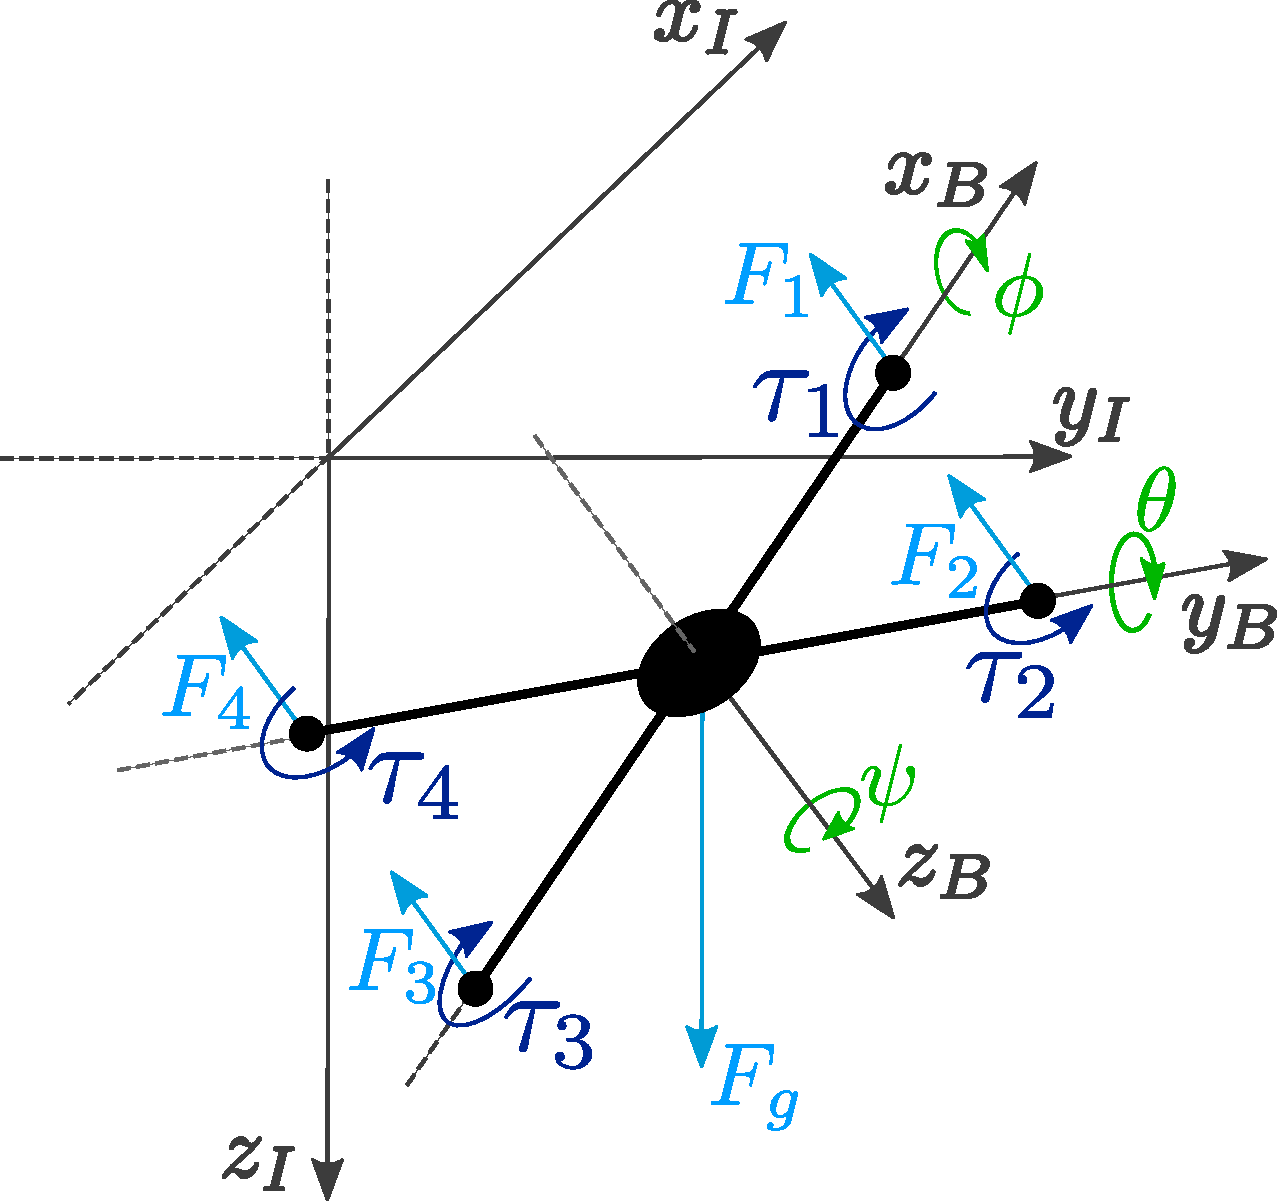
\includegraphics[scale=0.3]{figures/droneDiagram}
	\caption{Quadcopter diagram showing the forces and torques acting on the system and the positive references chosen for rotations and translations in both Inertial and Body coordinate frames.}
	\label{droneDiagram}
\end{figure}
The forces generated in the propeller are easily explained in the Body coordinate frame. In order to represent them in the Inertial frame a rotation matrix is used. It is built considering a 123 rotation sequence \cite{rotationmatrix}
 
The dynamic model of the quadcopter can be explain through three sets of equations. The first describes the motor and the propeller, the second presents the attitude response of the quadcopter and the third explains hos the translational variables of the system evolve with time.
\subsubsection{Motor and Propeller}
The four motors in the quadcopter generate the rotation required so the propeller creates the force that lifts the quadcopter. This force is called thrust force and can be modeled as proportional to the square of the motor rotational velocity. MAYBE SOURCE. The coefficient for this equation is called thrust coefficient and has been found by experiments.  
The rotation of the propellers also generates a torque on each motor due to drag between air and propeller. Drag torque is compensated in the quadcopter by having two of the motors turning in one direction and the two others in the opposite. It can also be described as proportional to the square of the velocity by terms of a drag coefficient that has also been obtained through tests.
Equation \ref{eq:thrustForce} and \ref{eq:dragTorque} show the expression for the thrust force and drag torque caused by the rotation of the propeller.
\begin{align}
	F&=k_{th}\omega^2\label{eq:thrustForce}\\
	\tau&=k_{d}\omega^2\label{eq:dragTorque}
\end{align}
\textbf{INCLUDE WHERE}\\
This equations are included in the attitude and translational models derived below.
\subsubsection{Attitude Model}
The attitude model equations are based on Newton Second Law for rotational movement and are represented in Equation \ref{eq:AngleEqVelocities1}, \ref{eq:AngleEqVelocities2} and \ref{eq:AngleEqVelocities3}. 
\begin{align}
	J_x\ddot{\phi}&=k_{th} (\omega^2_4-\omega^2_2)  L \label{eq:AngleEqVelocities1}\\
	J_y \ddot{\theta}&=k_{th} (\omega^2_1-\omega^2_3)  L \label{eq:AngleEqVelocities2} \\
	J_z\ddot{\psi}&=k_d (\omega^2_1-\omega^2_2+\omega^2_3-\omega^2_4)\label{eq:AngleEqVelocities3}
\end{align}
\textbf{INCLUDE WHERE}\\
%\begin{where}
%	\va{k_{th}}{is the thrust coefficients}{N\cdot s^2 \cdot rad^{-2}}
%	\va{k_d}{is the drag coefficients}{N \cdot m\cdot s^2 \cdot rad^{-2}}
%\end{where}
The expressions above state how the thrust force difference between motors 1 and 3 affects the roll angular acceleration, how that between motors 4 and 2 affects the pitch angle and how the yaw acceleration depends on the four motors by means of the drag torque generated on the propeller.  
\subsubsection{Translational Model}
The equations describing the response of the system along the x, y and z axes is derived from Newton's Second Law. The forces that act on the system are those from the propellers and the gravitational. These expressions are shown in Equation \ref{eq:AccelerationEqInertial1}, \ref{eq:AccelerationEqInertial2} and \ref{eq:AccelerationEqInertial3}. FIX EQUATIONS
\begin{flalign}
 	\eq{m\ddot{x}_I}{-k_{th}({\omega_1}^2+{\omega_2}^2+{\omega_3}^2+{\omega_4}^2)\sin(\theta)} \label{eq:AccelerationEqInertial1}\\
 	\eq{m\ddot{y}_I}{-k_{th}({\omega_1}^2+{\omega_2}^2+{\omega_3}^2+{\omega_4}^2)(-\sin(\phi))\cdot\cos(\theta)} \label{eq:AccelerationEqInertial2}\\
 	\eq{m\ddot{z}_I}{F_g-k_{th}({\omega_1}^2+{\omega_2}^2+{\omega_3}^2+{\omega_4}^2)\cos(\phi)\cdot\cos(\theta)}
 	\label{eq:AccelerationEqInertial3}
\end{flalign}
It is worth mentioning that, as the thrust forces always point in the negative z direction in the body coordinate frame, the accelerations in x and y directions in the inertial frame are zero as long as pitch and roll angles are 0.
\subsection{Linearization}
The linearization of the model equations has been developed following the first order Taylor approximation around an equilibrium point of the system. The chosen point is the hovering position and that implies that all variables have a value of zero, that is, the translational and attitude accelerations, velocities and positions. Choosing a zero acceleration equilibrium point along the Inertial z axis yields a equilibrium rotational speeds so that the necessary thrust is generated to compensate for the gravitational force.

The resulting equations for the attitude model after the linearization are shown in Equation \ref{eqAngleLin1}, \ref{eqAngleLin2} and \ref{eqAngleLin3}. 
\begin{flalign}
	J_x\Delta\ddot{\phi}   &= 2k_{th}L({\overline{\omega}_4} \Delta \omega_2-{\overline{\omega}_2} \Delta \omega_4)
	\label{eqAngleLin1} \\
	J_y\Delta\ddot{\theta} &= 2k_{th} L({\overline{\omega}_1} \Delta \omega_1-{\overline{\omega}_3} \Delta \omega_3) 
	\label{eqAngleLin2} \\
	J_z\Delta\ddot{\psi}   &= 2k_d({\overline{\omega}_1}\Delta \omega_1-{\overline{\omega}_2}\Delta \omega_2+{\overline{\omega}_3}\Delta \omega_3-{\overline{\omega}_4} \Delta \omega_4) \label{eqAngleLin3}
\end{flalign}
\textbf{INCLUDEWHERE}
%\begin{where}
%	\va{ \Delta\ddot{\phi}     } {is the change in roll angular acceleration from equilibrium}         { rad \cdot s^{-2} }
%	\va{ \Delta\ddot{\theta}   } {is the change in pitch angular acceleration from equilibrium}        { rad \cdot s^{-2} }
%	\va{ \Delta\ddot{\psi}     } {is the change in yaw angular acceleration from equilibrium}          { rad \cdot s^{-2} }
%	\va{ \overline{\omega}_i } {is the angular velocity of each motor in equilibrium}             { rad \cdot s^{-1} }
%	\va{ \Delta \omega_i       } {is the change in angular velocity from equilibrium of each motor} { rad \cdot s^{-1} }
%\end{where}
Similarly, the equations of the translational model are linearized. The result is shown in \ref{eq:TransLinearEquations1}, \ref{eq:TransLinearEquations2} and \ref{eq:TransLinearEquations3}. \textbf{FIX EQUATIONS}
\begin{flalign}
	m\cdot\Delta\ddot{x}_I &= -k_{th}({\overline{\omega}_1}^2+{\overline{\omega}_2}^2+{\overline{\omega}_3}^2+{\overline{\omega}_4}^2)\cos(\overline{\theta}) \Delta\theta \label{eq:TransLinearEquations1} \\
	m\cdot\Delta\ddot{y}_I &=  k_{th}({\overline{\omega}_1}^2+{\overline{\omega}_2}^2+{\overline{\omega}_3}^2+{\overline{\omega}_4}^2)\cos(\overline{\phi})\cos(\overline{\theta})\Delta\phi \label{eq:TransLinearEquations2}\\
	m\Delta\ddot{z}_I &= -2\textbf{ }k_{th}({\overline{\omega}_1}\Delta\omega_1+{\overline{\omega}_2}\Delta\omega_2+{\overline{\omega}_3}\Delta\omega_3+{\overline{\omega}_4}\Delta\omega_4)\cos(\overline{\phi})\cos(\overline{\theta})\label{eq:TransLinearEquations3}
\end{flalign} 
\textbf{INCLUDEWHERE}
%
%\begin{where}
%	\va{\Delta\ddot{x_I}  }{ is the change in linear acceleration from equilibrium in $x_I$ direction }{ m \cdot s^{-2} } \\
%	\va{\Delta\ddot{y_I}  }{ is the change in linear acceleration from equilibrium in $y_I$ direction }{ m \cdot s^{-2} } \\
%	\va{\Delta\ddot{z_I}  }{ is the change in linear acceleration from equilibrium in $z_I$ direction }{ m \cdot s^{-2} } \\
%	\va{\Delta \phi       }{ is the change in roll from equilibrium                          }{ rad            } \\
%	\va{\Delta \theta     }{ is the change in pitch from equilibrium                         }{ rad            } \\
%	\va{\Delta \psi       }{ is the change in yaw from equilibrium                           }{ rad            } \\
%	\va{\overline{\phi}   }{ is the roll in equilibrium                                      }{ rad            } \\
%	\va{\overline{\theta} }{ is the pitch in equilibrium                                     }{ rad            } \\
%	\va{\overline{\psi}   }{ is the yaw in equilibrium                                       }{ rad            }
%\end{where}}%\vspace{.5cm}
\end{alertblock}

%----------------------------------------------------------------------------------------

\end{column} % End of the first column

\begin{column}{\sepwid}\end{column} % Empty spacer column

\begin{column}{\twocolwid} % Begin a column which is two columns wide (column 2)


%----------------------------------------------------------------------------------------
%	CONTROL SOLUTION
%----------------------------------------------------------------------------------------
\begin{alertblock}{Control Solution\vspace{2pt}}
\subsection{Control}
The control of the system is divided into two control systems. One handles the attitude equations and the other controls the translational variables. 
\end{alertblock}
%----------------------------------------------------------------------------------------

%----------------------------------------------------------------------------------------
%	RESULTS
%----------------------------------------------------------------------------------------
\begin{alertblock}{Results\vspace{2pt}}
	\section{Results}
Simulation vs. reality. \\
%Design a setup that allows a nice measurement of reality - yet to be done\\
Comment on the results and how that correlates with reality, without discussing possible issues or improvements.
Model parameters: \fxnote{bring table with values}
Controllers:
Attitude controller:
Translational controller:

The inner loop proportional controller of the x and y translational cascade controllers are as follows:
\begin{align}
C_{\dot{x_I}}(s)= -0.19\\
C_{\dot{y_I}}(s)= 0.19
\end{align}

The outer loop  proportional controller of the x and y translational cascade are as follows:
\begin{align}
C_{\dot{x_O}}(s)&= 0.55\\
C_{\dot{y_O}}(s)&= 0.55
\end{align}

\end{alertblock} 

\end{column} % End of the second column

\begin{column}{\sepwid}\end{column} % Empty spacer column

\begin{column}{\onecolwid} % The third column

%----------------------------------------------------------------------------------------
%	Results
%----------------------------------------------------------------------------------------

%----------------------------------------------------------------------------------------

%----------------------------------------------------------------------------------------
%	DISCUSSION
%----------------------------------------------------------------------------------------
\begin{alertblock}{Discussion\vspace{2pt}}
\centering
\vspace{.5cm}
\parbox{.95\textwidth}{
\chapter{Discussion}
}\vspace{.5cm}
\end{alertblock}

%----------------------------------------------------------------------------------------
%	Conclusion
%----------------------------------------------------------------------------------------
\begin{alertblock}{Conclusion\vspace{2pt}}
\centering
\vspace{.5cm}
\parbox{.95\textwidth}{
\section{Conclusion}
In this project, the behavior of a quadcopter has been modeled by first principles of physics. A control system has been designed in order to hover and move to a desired position.
The control system has been split into an attitude and a translational controller. The first one has been designed using a state space approach, including state feedback with integral control and a reduced order observer. The translational control system has been designed with a classical control approach and result in three cascade loops, including proportional and PI controllers. 
As the quadcopter uses an external motion tracking system to determine its position and orientation, an analysis of the issues that can arise when having a networked distributed system has been done in order to ensure the control system remains stable. The performance of the controllers shown in the results demonstrates the efficiency of the control strategy reveal in the paper.


}\vspace{.5cm}
\end{alertblock}

%----------------------------------------------------------------------------------------
%	References
%----------------------------------------------------------------------------------------
\begin{alertblock}{References\vspace{2pt}}
\centering
\vspace{.2cm}
\parbox{.98\textwidth}{
\nocite{FeedbackControl} % Insert publications even if they are not cited in the poster
\nocite{TrueTimeNew}
\printbibliography
}\vspace{.2cm}
\end{alertblock}

%----------------------------------------------------------------------------------------
%	Acknowledgements
%----------------------------
\begin{alertblock}{Acknowledgements\vspace{2pt}}
\centering
\vspace{.2cm}
\parbox{.98\textwidth}{
Henrik Shøiler, Associated Professor, Aalborg University.
}\vspace{.2cm}
\end{alertblock}

%----------------------------------------------------------------------------------------

\end{column} % End of the third column

\end{columns} % End of all the columns in the poster

%\tikz[remember picture,overlay] \node[opacity=0.7,inner sep=0pt] at (current page.center){
\includegraphics[width=\paperwidth,height=\paperheight]{figures/drawing}};
%\clearpage
\end{frame} % End of the enclosing frame

\end{document}
